\chapter{Targeting the Non-Excluded pMSSM with Multivariate Discriminants}
\label{chap:money}
\FloatBarrier

Designing analyses to target the non-excluded regions of the pMSSM is challenging for a number of reasons. The fact that the signal events in this subset contain soft objects and low $\met$ means that the observables typically used to distinguish between \SM~backgrounds and the signal no longer function as excellent discriminators. 

However, the situation is not completely dire. The  $\Ht$, $\met$, and the prevalence of high $p_{T}$ objects are popular largely because they exploit relatively well-understood differences between typical new physics signals and background. There are presumably other aspects of collision events that may differ between events arising from supersymmetry those from standard model processes, such as the relative angles between particles, the presence and characteristics of leptons and heavy-flavor quarks in the events, certain Lorentz invariant event properties, as well as various combinations of the four-vectors of particles. Information not considered in most searches, but to which we have ready access, include the $\pt$, $\eta$, and $\phi$ of particles in the event. Correlations among these observables may serve to distinguish between $\sm$ events and BSM events.

This brief chapter combines all of the methods presented in this document into a demonstration of a battle strategy for targeting non-excluded SUSY models that predict large cross sections in the most challenging, all-hadronic kinematic regions: low $\met$, where QCD is the dominant background, and low $\Ht$, where $\zinv$ events are the largest background. Chapter \ref{chap:run1pmssm} demonstrated that these regions may constitute pay dirt. 

\subsection{New observables and new events; same methods}
Can our sensitivity to the pMSSM be increased through the use of multivariate discriminants? Addressing a few questions is key in order to proceed: 
\begin{enumerate}
\item Does the collection of particle four-vectors actually contain information that distinguishes signal events from background events?
\item Can this information be accurately modeled in real and simulated events?
\item Is any such discrimination power generalizable to a large class of interesting models, or is it limited to a narrowly-defined subset of models or even a single model?
\end{enumerate}
I set out to answer these questions by considering events in two background-dominated kinematic signal regions, corresponding to modified versions of the CMS multi-jet $+$ $\mht$ search's \cite{Khachatryan:2016kdk} baseline selection. The fist signal region is taken to be the low-$\mht$ sideband of the \cite{Khachatryan:2016kdk} baseline selection where the range $\mht=150$$-$$200$ GeV is considered, and the second is the taken to be the low-$\Ht$  sideband, such that events in the range $\Ht=400$$-$$500$ GeV are considered. In each signal region, a separate multivariate discriminant is trained and tested, making full use of the data-driven background estimation methods described earlier. I give myself two chances to answer questions 1$-$3, one for each signal region.

\subsection{Low-$\mht$ discriminant}
The kinematic region defined by the range $\mht=150$$-$$200$ GeV is largely dominated by QCD multi-jet events. Therefore, I focus on rejecting QCD events while accepting hypothetical SUSY events by following this strategy.
\begin{itemize}
\item Create a pure sample of QCD events using the data-driven QCD generator based on the rebalance and smear method (Section \ref{sec:qcd});
\item obtain a few samples of SUSY signal events corresponding to models that are nearly excluded by the existing CMS searches (I consider SUSY models within the SMS framework, T1qqqq with $m_{\tilde{\text{g}}}=1000$ GeV and $m_{\tilde{\chi}^{0}_{1}}=800$ GeV,  T1bbbb with $m_{\tilde{\text{g}}}=1000$ GeV and $m_{\tilde{\chi}^{0}_{1}}=900$ GeV, and T1tttt with $m_{\tilde{\text{g}}}=1200$ GeV and $m_{\tilde{\chi}^{0}_{1}}=800$ GeV);
\item train a discriminant using the QCD sample for the background events, and pooled events from the three SUSY models for the signal training events;
\item observe the accuracy of the modeling of the discriminant output in an independently simulated set of QCD and signal events, and
\item observe potential sensitivity to a range of signal models.
\end{itemize}

A boosted decision tree is trained using the signal and background samples, taking the $\pt$, $\eta$, and $\phi$ of each of the four leading jets, as well as the $\mht$, $\Ht$, and $\njets$ as inputs. The output of the discriminant for signal and background is shown in Fig. \ref{fig:SusyBdt}. The modeling of the QCD background in simulation by the rebalance and smear method is shown in Fig. \ref{fig:SusyBdt}, overlaid with the distribution of a few signal model points. Agreement to within a few percent is observed between the prediction and expectation, evidence that the Bayesian rebalance and smear method can accurately model the correlations of up to 15 observables. Also shown are the distributions of the BDT output for the three chosen signal models, as well as a graph showing the tradeoff between the signal efficiency and background rejection (ROC curve). Additional discrimination achieved through multivariate discriminants, which are successfully modeled modeled using a data-driven method lain out in this document. The discriminants achieve greatly increased sensitivity to a broad class of models.
\begin{figure}[tb!]
\centering
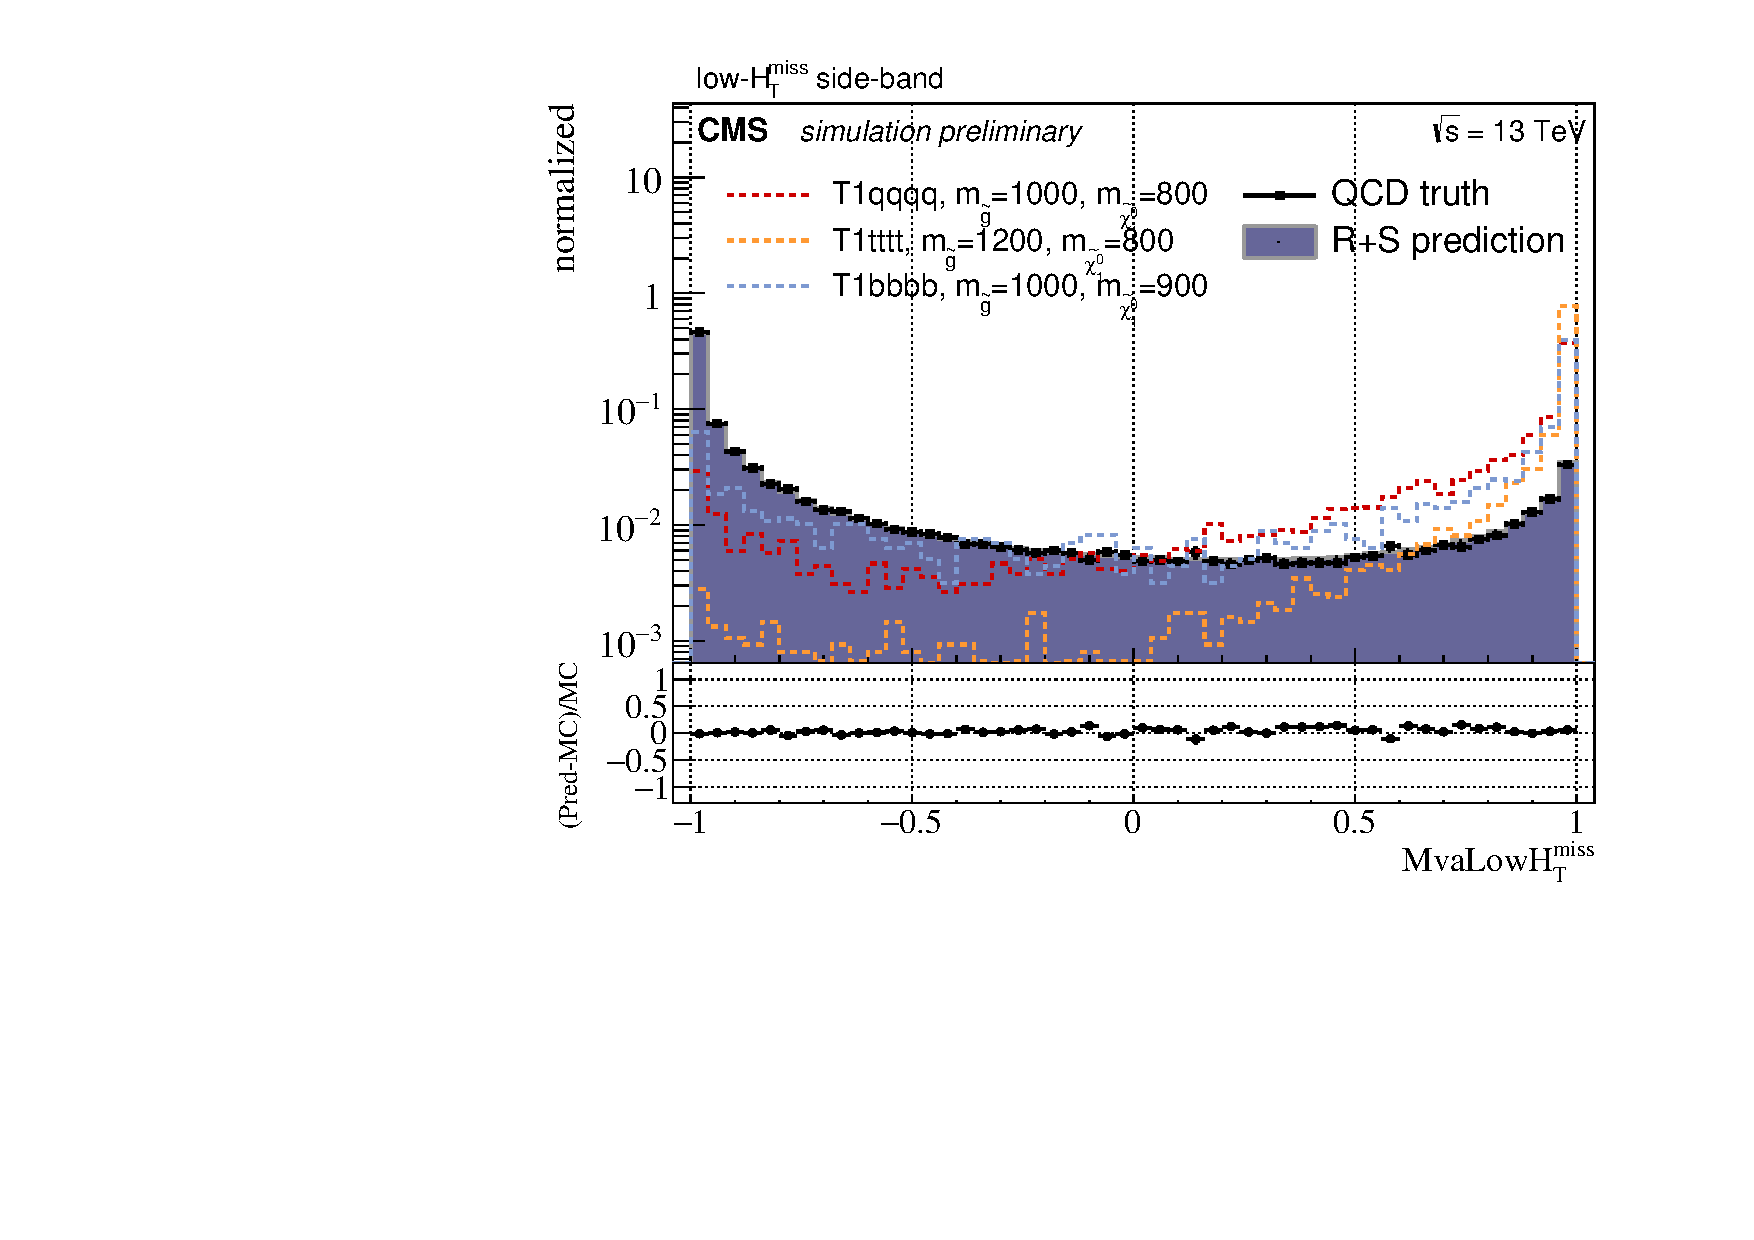
\includegraphics[width=0.7\linewidth]{figures/SusySearches/MvaLowMht.pdf}
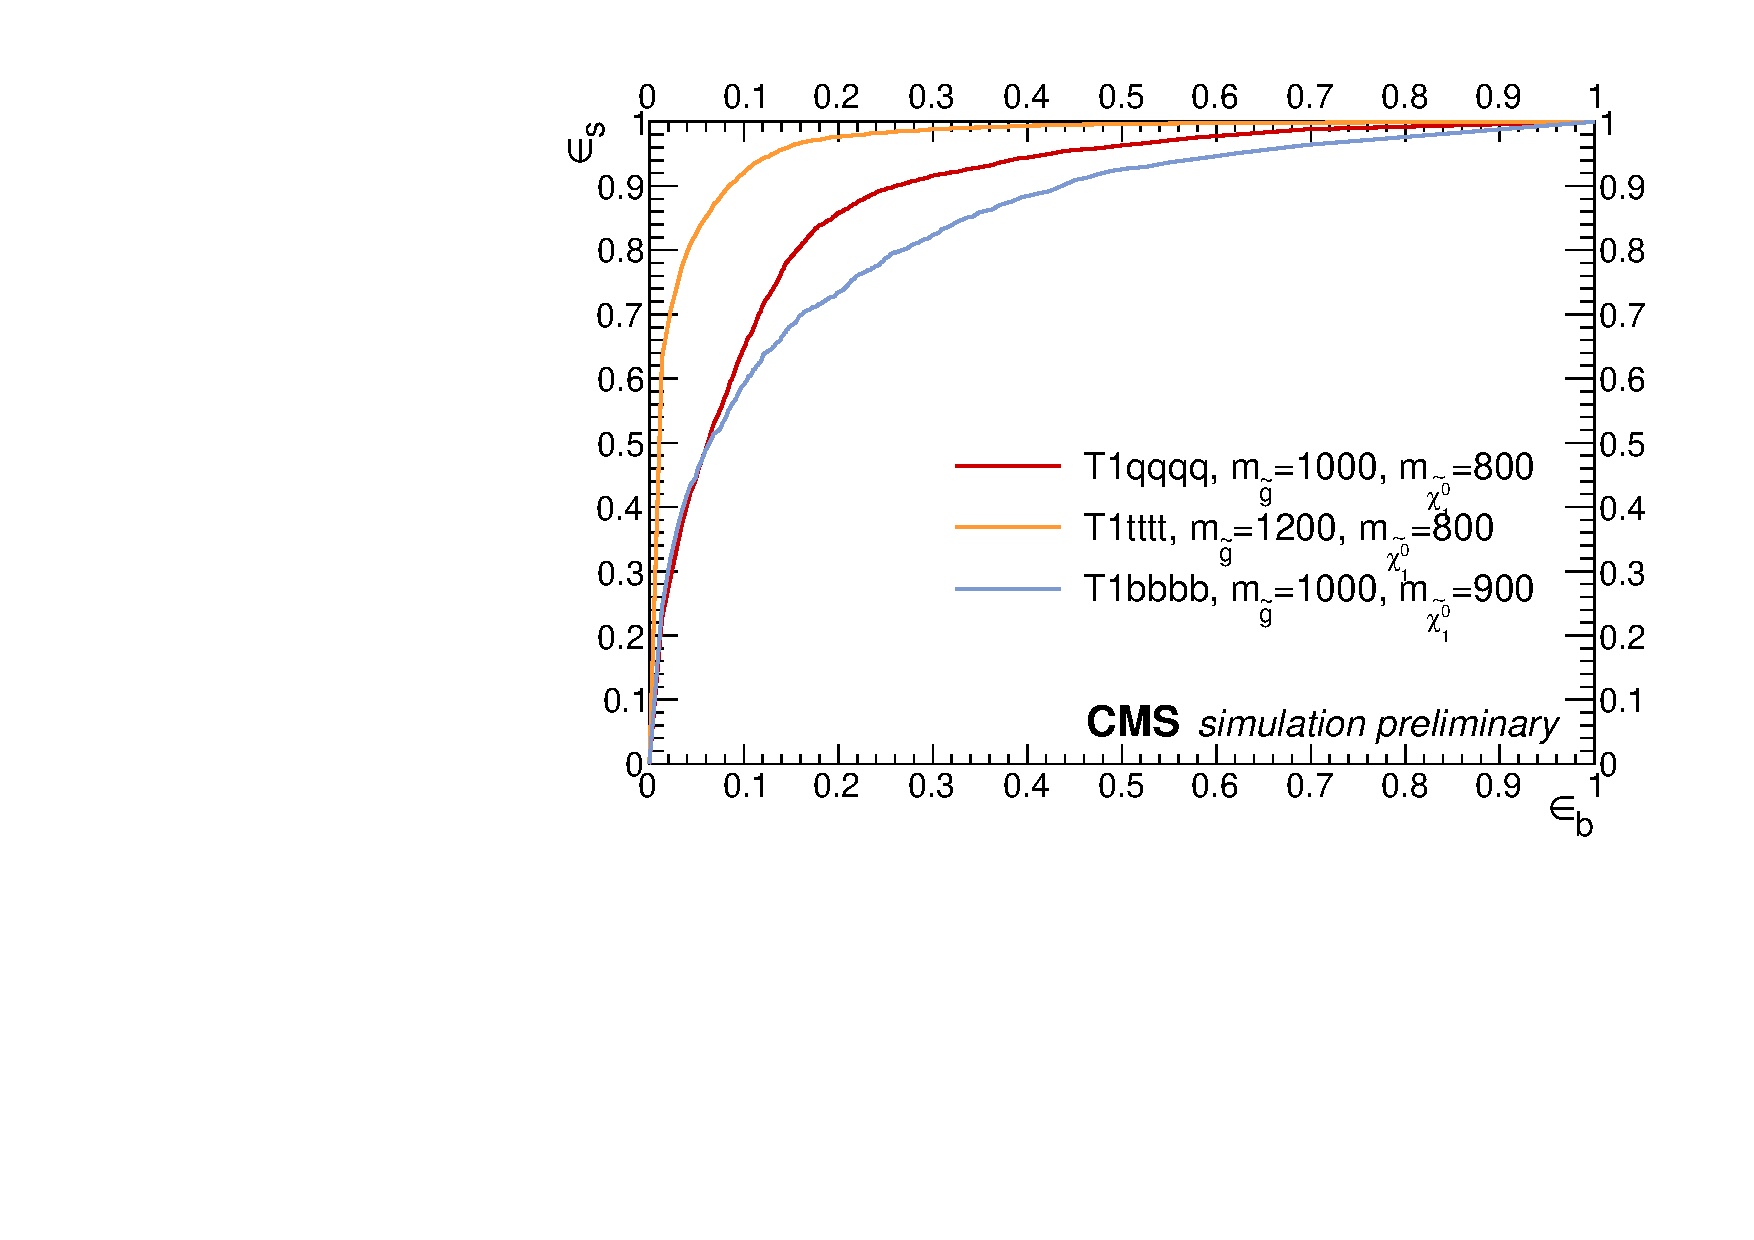
\includegraphics[width=0.7\linewidth]{figures/SusySearches/RocCurvesLowMht_QCDVsSUSY.pdf}
\caption{Top: the distribution of the output of the low-$\mht$ data-driven discriminant for a sample of simulated QCD events, compared with the distribution obtained by applying the rebalance and smear method to simulation. Also shown are the distributions of the output for a few signal points corresponding to various SMS scenarios. Bottom: the efficiency of selecting signal events vs that of selecting background events, based on a scan through all possible thresholds on the discriminant.}
\label{fig:SusyBdt}
\end{figure}

\FloatBarrier
\subsection{Low-$\Ht$ discriminant}
A similar procedure is applied in the low-$\Ht$ signal region. In this region, the dominant standard model Model background is from the production of $Z$ bosons in association with jets, where the $Z$ decays into neutrinos. Therefore, I focus on rejecting $\zinv$ events while accepting SUSY signal events with high efficiency. Using the data-driven $\zinv$ background estimation methods described in Section \ref{sec:zinv}, and continuing the approach of using real data samples for the background training evebs for multivariate discriminants, the following strategy is taken.
\begin{itemize}
\item Obtain a $\zinv$ prediction sample based on a real sample of $\zmumu$ events that have been cleaned of muons and reweighted to account for inefficiencies of lepton selection (as described in Section \ref{sec:zinv});
\item obtain the same samples of SUSY signal events used earlier, namely, T1qqqq with $m_{\tilde{\text{g}}}=1000$ GeV and $m_{\tilde{\chi}^{0}_{1}}=800$ GeV,  T1bbbb with $m_{\tilde{\text{g}}}=1000$ GeV and $m_{\tilde{\chi}^{0}_{1}}=900$ GeV, and T1tttt with $m_{\tilde{\text{g}}}=1200$ GeV and $m_{\tilde{\chi}^{0}_{1}}=800$ GeV);
\item train a multivariate discriminant using the $\mu\mu$-derived $\zinv$ prediction sample for the background events, and the  SUSY model point for the signal events;
\item observe the accuracy of the modeling of the discriminant output using the data-driven prediction applied in simulation to the dielectron sample compared with direct $\zinv$ simulation, and
\item observe potential sensitivity to the signal models.
\end{itemize}
The modeling of the BDT output distribution for a simulated sample of $\zinv$ events is shown in Fig. \ref{fig:SusyBdt2}, along with the distribution for the sample obtained by applying dielectron prediction method to $\zee$ simulation. Overlaid with these distributions are distributions of the chosen signal model points. Once again, significant sensitivity increases are achieved through multivariate discriminants across a range of SUSY models, and the discriminant are accurately modeled by the data-driven methods developed herein. 
\begin{figure}[tb!]
\centering
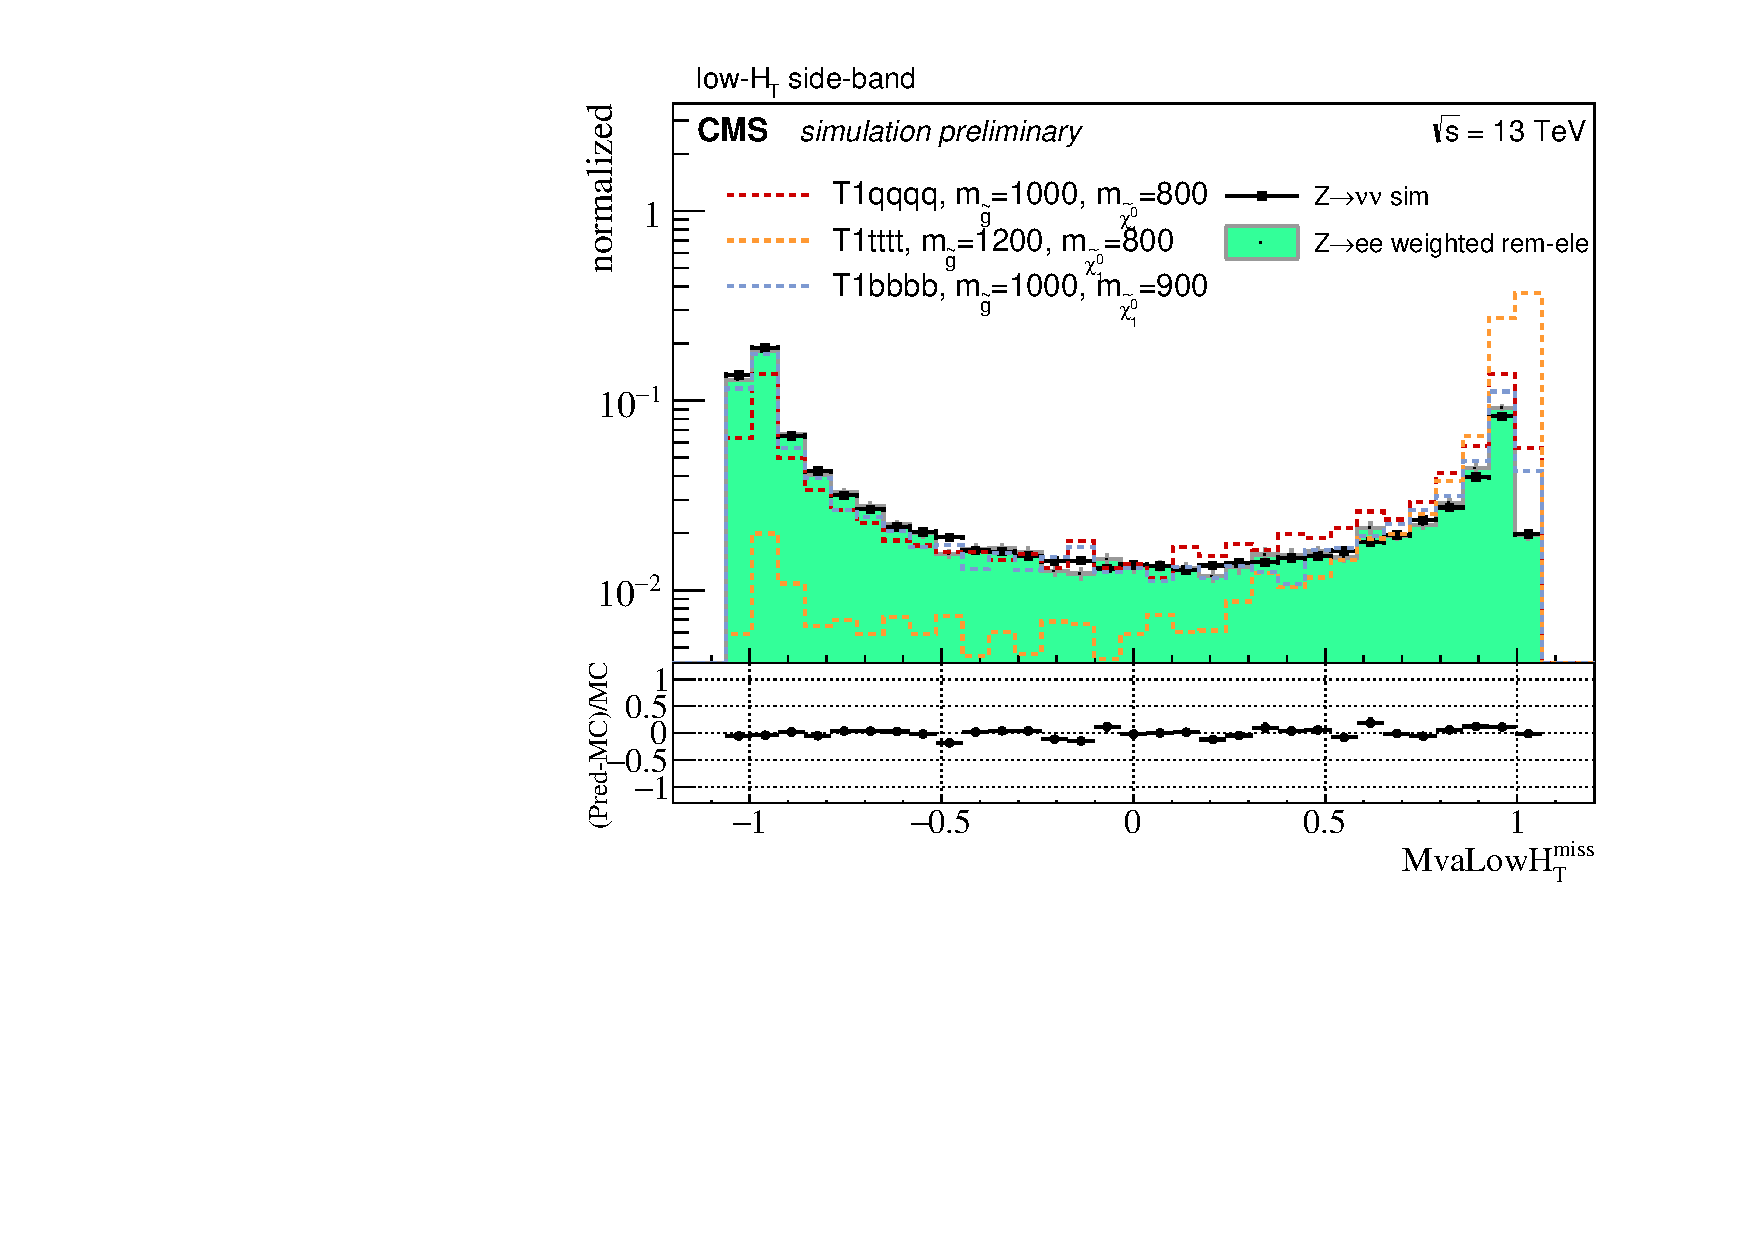
\includegraphics[width=0.7\linewidth]{figures/SusySearches/MvaLowHt.pdf}
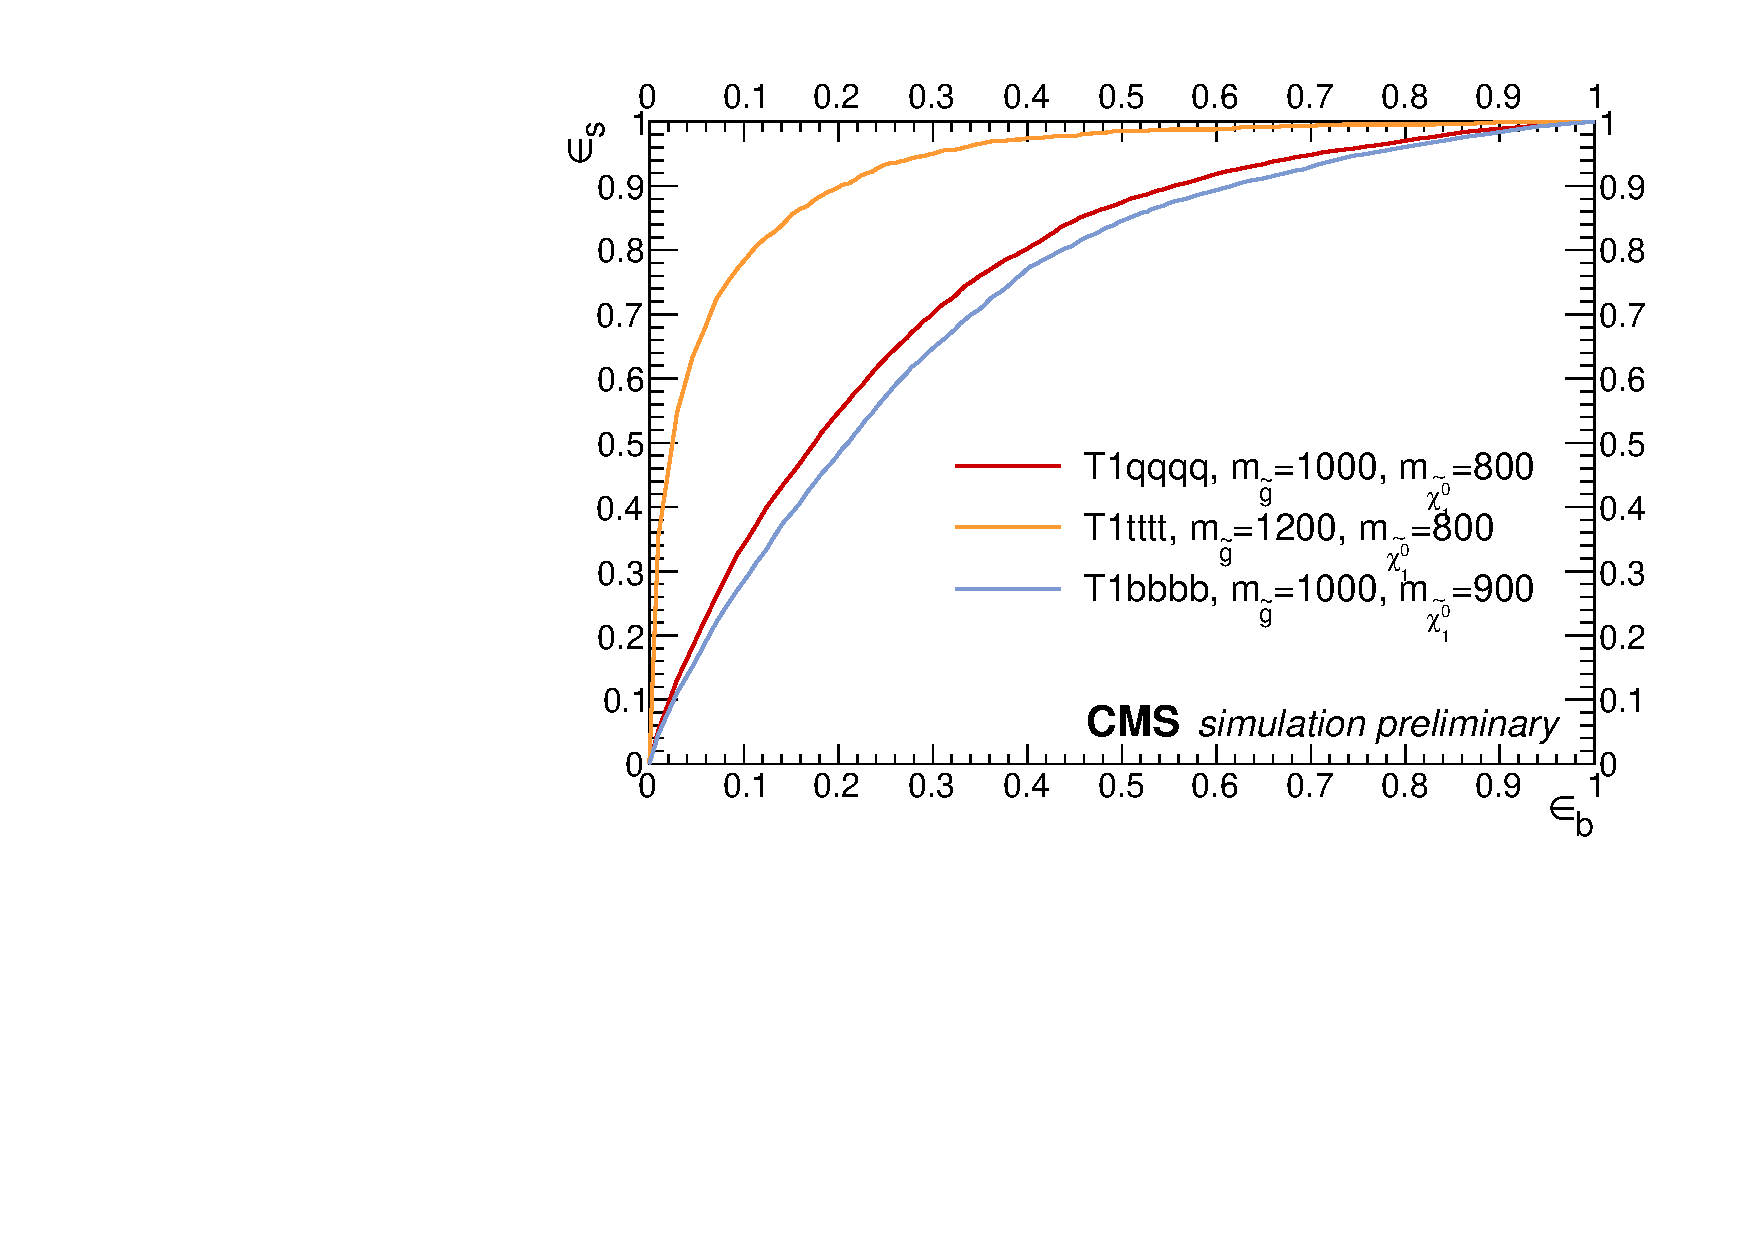
\includegraphics[width=0.7\linewidth]{figures/SusySearches/RocCurvesLowHt_ZinvVsSUSY.pdf}
\caption{Top: The distribution of the output of the low-$\Ht$ muon data-driven multivariate discriminant for a sample of simulated $\zinv$ events, compared with the distribution obtained by applying the data-driven dielectron prediction method to simulation. Also shown are the distributions of the output for a few signal points corresponding to various SMS scenarios. Bottom: the efficiency of selecting signal events vs that of selecting background events, based on a scan through all possible thresholds on the discriminant.}
\label{fig:SusyBdt2}
\end{figure}

\subsection{Potential future work}

Events ought to be collected with a trigger like the monojet trigger discussed in Section \ref{sec:anatrig}. The trigger efficiency has been measured using the single-electron sample and multivariate probability estimator discussed in Section \ref{sec:anatrig}. 

The signal samples chosen here pertain to simplified SUSY models. Ideally, nonexcluded pMSSM signal events can be used to train future discriminants. The exact procedure for how to pool the signal events from the pMSSM points to achieve good sensitivity to broad regions of the nonexcluded subspace should be developed. As shown, an unweighted pooling of signal events from different models can result in a discriminant that performs well over all models. 

A suggested procedure is to train a multivariate discriminant for each domain of the pMSSM model space, where a domain is defined as the set of points corresponding to a single principal process (Chapter \ref{chap:run1pmssm} Section \ref{sec:unexplored}, particularly Fig. \ref{fig:diagrams1}). For each discriminant, either an unweighted pooling of signal events can be used in the training, or alternatively, events could be weighted by the Z-signficance of the pMSSM points, or by the cross section. Studies would be required to optimize this procedure.

It is possible that providing more sophisticated variables as input to a multivariate discriminate could result in better performance than that achieved by the discriminants discussed here. Appendix \ref{app:discriminators} gives a brief introduction to a few such observables, some of which have been central to CMS and/or ATLAS searches for supersymmetry. Studies that evaluate the effectiveness with which these observables probe the pMSSM, taken alone and in combinations with each other, may prove informative.




